\documentclass[10pt,a4paper]{article}
\usepackage[utf8]{inputenc}
\DeclareUnicodeCharacter{00A0}{~}  % or not it by utf8x
\usepackage[T4]{fontenc}
\usepackage[polish]{babel}
%\usepackage {polski}
\let\lll\undefined
\usepackage{amssymb,amsmath,amsthm}
\usepackage[breaklinks]{hyperref}
\usepackage{graphicx}
\marginparwidth=5.2cm \hoffset=2.5cm \textwidth=12.5cm
\textheight=25.2cm \reversemarginpar \voffset=-1in
%\addtolength{\textheight}{2in}

% Moje pliki latexowe artykułów, które napisałem mają mniej więcej 1100 - 1600 słów
% i to jest trochę ponad 2 strony. A więc celuj w 1000 słów (lub 500 - na 1 stronę), a jak przekroczysz
% to nic się nie stanie. Objętość tekstu nie jest taka ważna, ważniejsza jest treść ;).

\begin{document}
%tytuł
\noindent\textbf{\LARGE Prawdopodobieństwo a informacja}

\medskip
%autor
\noindent\textit{\Large Piotr Migdał}
\marginpar{\footnotesize
    *dr z ICFO--The Institute of Photonic Sciences, Castelldefels (Barcelona), obecnie freelancer z analizy danych \url{http://migdal.wikidot.com}}

\medskip

O ile entropia jest używana w języku potocznym jako chaos i nieuporządkowanie, to sama wielkość jest ściśle określonym pojęciem --- \emph{informacją Shannona}:
%
    \marginpar{\footnotesize Cześciej jest pisane w sumie $-p_i \log(p_i)$ --- równoważnie ale, moim zdaniem, mniej dydaktycznie.}
%
\begin{align}
    H = \sum_{i=1}^{n} p_i \log \left(\tfrac{1}{p_i} \right),\label{eq:entropia}
\end{align}
%
    \marginpar{\footnotesize Korzystatnie z innej podstawy logarytmu, np. $e=2.718\ldots$ przemnoży wynik przez stałą, a zatem odpowiada tylko zmianie jednostek: $\ln(x)=\ln(2)\log_2(x)$. Np. dla podstawy $e$ jednostką jest \emph{nit}.}
%
gdzie $\{p_1, \ldots, p_n\}$ to pewien rozkład prawdopodobieństwa.
Będziemy używać podstawy logarytmu $2$, co odpowiada mierzeniu entropii w \emph{bitach}.
Powyższy wzór ma wiele zastosowań i interpretacji.

Ale zanim przejdziemy do nich, spójrzmy na kilka prostych przykładów.
Gdy nasz rozkład składa się z jednej możliwości, entropia wynosi $0 \log(1) = 0$ bitów --- wszak nie ma tu miejsca na losowość.
Gdy rzucamy uczciwą monetą, entropia to $\tfrac{1}{2} \log(2) + \tfrac{1}{2} \log(2) = 1$ bit.
Entropia jest największa, gdy dla ustalonej liczby zdarzeń wszystkie są równo prawdopodobne --- wtedy entropia to $\log(n)$.
Dla kostki do gry z $6$ ścianami to $\log(6)\approx 2.6$.

Warto pamiętać, że entropia jest zawsze miarą niewiedzy.
Stąd np. kostka, na której widzimy wyrzucone dwa oczka ma entropię zero.
Dowiadujemy się dokładnie tyle, o ile entropia zmalała, tu:
%
\begin{align}
 H(\tfrac{1}{6}, \tfrac{1}{6}, \tfrac{1}{6}, \tfrac{1}{6}, \tfrac{1}{6}, \tfrac{1}{6}) - H(0, 1, 0, 0, 0, 0) = \log(6) - \log(1) \approx 2.6.
\end{align}
%
Gdyby ktoś nad powiedział wypadło jedno, dwa lub trzy oczka, nasz wiedza końcowa byłaby niepełna i dowiedzielibyśmy się $\log(6) - \log(3) = 1 $ bit informacji.


    \marginpar{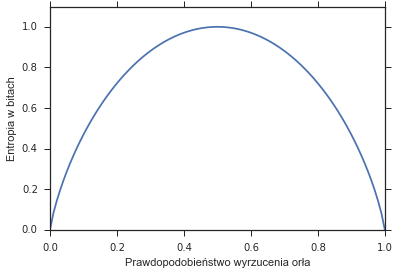
\includegraphics[height=3.5cm]{entropia2}\\
    \footnotesize Entropia rzutu obciążoną monetą.}

    % \marginpar{\footnotesize Z matematycznego punktu widzenia $\lim_{p \to 0} p \log(p) = 0$, z fizycznego --- nie chcemy by dodanie nierealistycznej opcji (tj. z zerowym prawdopodobieństwem) zmieniało wynik.}

Dlaczego potrzebujemy w tym wzorze logarytmu? 
Gdy mamy dwa niezależne zdarzenia, chcemy by ich entropia była sumą entropii składników.
Powedzmy, że chcemy dowiedzieć się jaki jest znak zodiaku naszego obiektu westchnień oraz czy nas kocha.
Nie powinno grać roli czy dowiemy się na raz jednej informacji czy po kawałku.
Oznaczymy prawdopodobieństwa znaków zodiaku jako $\{p_1, \ldots, p_{12} \}$ oraz uczucie do nas jako $\{q_1, q_2\}$.
Tym samym prawdopodobieństwa poszczególnych zdarzeń to iloczyny: $p_i q_j$.
Zatem jak z entropią?
%
    \marginpar{\footnotesize Czytelnikowi, który zastanawia się czy owe dane są niezależne, polecam zapoznać się z \url{http://bit.ly/dating-zodiac}.}
%

\begin{align}
    \sum_{i=1}^{12} \sum_{j=1}^2 p_i q_j \log(1/(p_i q_j))
    &= \sum_{i=1}^{12} \sum_{j=1}^2 p_i q_j \left( \log(1/p_i) + \log(1/q_j) \right)\\
    &= \sum_{i=1}^{12} \sum_{j=1}^2 p_i q_j \log(1/p_i)
    +\sum_{i=1}^{12} \sum_{j=1}^2 p_i q_j \log(1/q_j)\\
    &= \sum_{i=1}^{12} p_i \log(1/p_i)
    + \sum_{j=1}^2 q_j \log(1/q_j)
\end{align}
%
W szczególności $n$ rzutów uczciwą monatą to $n$ bitów bitów entropii.
%
    \marginpar{\footnotesize Wnikliwy czytelnik może sprawdzić, że też $-\log \sum_{i=1}^n p_i^2$ ma tę własność.
    I ogólnie cała rodzina \emph{entropi Rényi}, będących uogólnieniem entropii Schannona;
    przy czym w ogólności nie mają one interpretacji jako informacja.}
%
Na wzór na entropię Shannona można patrzeć również jak na średnią informację.
Dlaczego można traktować $\log(1/p)$ jak cokolwiek zwiazanego z informacją?
Bo gdy mamy kilka równoprawdopodobnych zdarzeń, każde zachącące z prawdopodobieństwem $p$,
to potrzebujemy $1/p$ bitów informacji by je odróżnić (każdy bit podwaja liczbę zdarzeń, które możemy rozróżnić).

[MOŻE TU SZERZEJ I BARDZIEJ W STRONĘ 20 PYTAŃ?]

Dobrze, ale dlaczego branie średniej ma sens?
Cóż, to jest treść twierdzenia Shannona, które mówi, że jeśli mamy ciąg liter,
każda niezależna od innych, to nie możmemy średnio skompresować bardziej niż do długości $n H$.
%Z drugiej strony kody Huffmana pozwalają skompresować dość blisko $n H$,

O ile stoją za tym pewne szczegóły techniczne, główną ideę można oddać zliczając ciągi.
Liczba słów o długości $n$ nad alfabetem z $d$ literami to $d^n=2^{n \log(d)}$.
Jeśli chcielibyśmy zakodować owe słowa przy pmocy zer i jedynek,
by każde słowo miało swój kod binarnym, potrzebujemy $m = n \log(d)$ bitów.
A co jeśli nie wszystkie litery są równie często używane?
Przede wszystkim, niektóre ciągi staną się skrajnie mało prawdopodobne.
Możemy wprowadzić kody o zmiennej długości, by częstsze ciągmi miały krótki kod.

Dla zwrócenia uwagi, zróbmy to na ciągu z zero i jedynek, z prawdopodobieństwami $p$ i $q$, odpowiednio.
Typowy ciąg o długości $n$ (gdzie $n$ jest duże) będzie miał $n p$ zer i $n q$ jedynek.
Prawdopodobieństwo tego ciągu to $p^{n p}q^{n q}$.
Można pokazać, że nietypowych ciągów jest bardzo mało, a zatem liczba typowych ciągów to:
$p^{-n p}q^{-n q}$.
Czyli, potrzebujemy
%
\begin{align}
    m=n \left( p \log(\tfrac{1}{p}) + q \log(\tfrac{1}{q}) \right)
\end{align}
%
bitów.
Innym słowem, liczba typowych ciągów rośnie jak $2^{n H}$.


I jeszcze jedno praktyczne zastosowanie entropi Shannona, tu --- do gry w \emph{20 pytań}.
Chcemy zadać pytanie, z którego odpowiedzi najwięcej wynika.
Możemy zapytać ``Czy to jest żywe?'', gdzie mamy z grubsza pół-na-pół szanse, że usłyszymy ``tak'' lub ``nie''.
Zatem zadając takie pytanie, dowiadujemy się
%
\begin{align}
    \tfrac{1}{2} \log(2) + \tfrac{1}{2} \log(2)  = 1
\end{align}
%
czyli jeden bit informacji. 
A może warto zadać pierwsze pytanie ``Czy chodzi o krzeszło?''?
Wtedy z jednej strony jest mała szansa usłyszenia ``tak'' (powiedzmy, $1/1024$),
niemniej gdy takowa odpowiedź padnie dostaniemy sporo informacji  ($-\log(1/1024)=10$).
Jednak średnio po uzyskaniu odpowiedzi dostaniemy
%
\begin{align}
    \tfrac{1}{1024} \log(2014) + \tfrac{1023}{1024} \log(\tfrac{1024}{1023}) \approx 0.01
\end{align}
%
bita, czyli niewiele.
Rzecz jasna, czasem nam nie zależy na średniej --- choćby gdy mamy 20.
Pytanie i urządza nas zgadnięcie, a nie tylko --- dojście bliżej.

Z pytań do zastanowienia się, jaką entropię mają:
\begin{itemize}
    \item ...kolejność talii 52 kart?
    \item ...litery w języku polskim?
    \item ...dwa zdarzenia, które są zależne --- większą czy mniejszą niż suma?
\end{itemize}


\section{Propozycje na kolejne odcinki}

\begin{itemize}
    \item Informacja wzajemna
    \item Inne entropie i liczenie różnorodności
    \item Temperatura
\end{itemize}


    \marginpar{\footnotesize  Lektury:\\
    Cosma Schalizi, Information theory\\
    \url{http://bactra.org/notebooks/information-theory.html}
    \url{http://mathoverflow.net/questions/146463/what-is-entropy-really}\\
    Dissecting the GZIP format\\
    \url{http://www.infinitepartitions.com/art001.html}}

\end{document}
